%% ==============================================
%%               FUNDAMENTALS
%% ==============================================
%% Author: Fabian Sorn
%% ==============================================

\chapter{Fundamentals}
\label{ch:fundamentals}

This chapter will give an introduction into the fundamental topics that are
relevant for the context of this work. In the first section we will have a look
at data visualization in general. We will start with a short exploration of the
development in history leading to our modern usage of data visualization in the
world of computing. Further we will explore a model which describes in general
the functionality and steps of modern data visualization frameworks and the
different types of data visualization applications. Finally the chapter will
present different usages of data visualization applications at \gls{cern}, which
different scenarios exist and what solutions are offered at the moment from the
\gls{aps} section.  In the second chapter we will move our focus on the topic of
performance benchmarking First, we will explore the different types of
benchmarks that exist on the market and followed by an introduction, how UI
performance can be benchmarked.  Since the focus of our benchmarking framework
will focus on applications using Qt and its python bindings, we will have a look
at its fundamental principles in the third section, which we will have to know
about, if we want to understand the performance of graph widgets written for it.
The fourth and last section of this chapter will give an introduction into
PyQtGraph, the plotting library of choice in \gls{aps} and the adaptions we are
developing for it in \gls{aps}.




%% ==============================================
%%             Data Visualization
%% ==============================================

\section{Data Visualization}
\label{sec:fundamentals:charting}

The following chapter gives a brief introduction into the history and
development of data visualization, presents a model which describes modern data
visualization frameworks and explores the usage of data visualization at CERN.


%% ==============================================
%%     The Development of Data Visualization
%% ==============================================

\subsection{The development of Data Visualization}
\label{sec:fundamentals:charting:history}

Good visualization helps us to understand patterns, trends and relationships in
data much more easily and share discoveries with others. Representing data in a
visual way has its root in the earlies of humanities history, where drawings on
cave walls were a way to share stories, which's marks we can still find
preserved until today. From there the idea of visualizing information, which we
want to share, evolved into many different directions. One very early way to
present data to viewers, was to use tables. The oldest preserved documents
presenting data in tables can be dated back to the 2nd century AD. Even though
the information was still presented mainly in text, alignment, whitespaces and
lines, were already utlized to support the viewer to navigate through data in
large quantities.  Visualizing data in a two dimensional space using a system of
coordinates has its roots in the 17th century. The two dimensional carthesian
coordinate system was the basis for displaying data as graphs. In the following
18th and 19th century more types of graphs like Bar Graphs and Pie Charts
emerged, which we still use in modern representations of datasets today.
\cite{DataVisHistory}

Visualization does not only help us in understanding static data, but also
discovering trends in its development over a period of time. In 1753, Jacques
Barbeu-Dubourg created a graph disaplying a large historical time line, called
the Carne Chronographique. The graph displays events from a total time span of
6480 years, drawn by hand on a 54 foot long paper roll. Entries are listed
chronologically behind each other from left to right. Special about this paper
roll was, that it visualizes a big amount of historical data, while keeping a
small form factor, which is achieved, by rolling the large paper onto a scroll.
Both parts of the scrolls were connected to keep always the same exact distance
to each other, presenting the Viewer view on a part of the entire data. To move
the timespan of this detailed view you could simply roll the paper further into
one direction to go back or forward in history.  \cite{DataVisHistPresentation}

\begin{figure}[h]
    \centering
    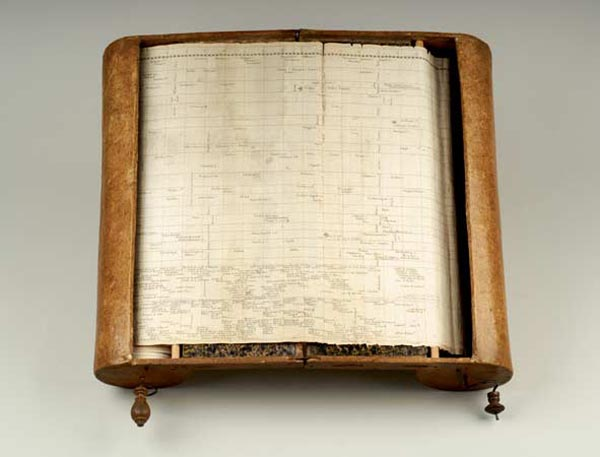
\includegraphics[width=12cm]{resources/img/ScrollOfHistory}
    \caption{Jacques Barbeu-Dubourg's Scroll of History}
    \small\textsuperscript{Quelle: https://earlyamericanists.files.wordpress.com/2015/05/chronographie-universelle.jpg}
    \label{fig:historyscroll}
\end{figure}

With the invention of computers and the rise of more affordable models in homes
and offices, data could be visualized much faster and easier then ever before.
The labor intensive process of drawing graphs by hand on special paper was
replaced by computer generated ones that could be created with the click of a
button. This drastic improvement in ease of use further increased the popularity
of data visualization and brought it into many more fields.
\cite{DataVisHistory2}

One of these areas was the integration of interactive graphs into \glspl{gui}.
No matter what language is chosen by a developer to write \gls{gui}
applications, chances are high that there alrady exist powerful libraries for
visualizing data. Compared to printed charts and graphs, graphs in software can
be a much more powerful tool, since they do allow the user to interact with
their data and and alter its visual representation. Additionally graphs
displayed on a screen can be updated when new data is available compared to
printed ones. A model which describes the functionality of such libraries, is
the Data Visualization Pipeline.  \cite{VisIdioms}




%% ==============================================
%%        Data Visualization Pipeline
%% ==============================================

\subsection{Data Visualization Pipeline}
\label{sec:fundamentals:charting:pipeline}

The Data Visualization Pipeline describes the transformation of raw data to a
visual representation of this data which can be displayed on a screen. This
transformation is achieved through a sequence of four operations that are
executed to transform the data step by step. 

\begin{figure}[h]
    \centering
    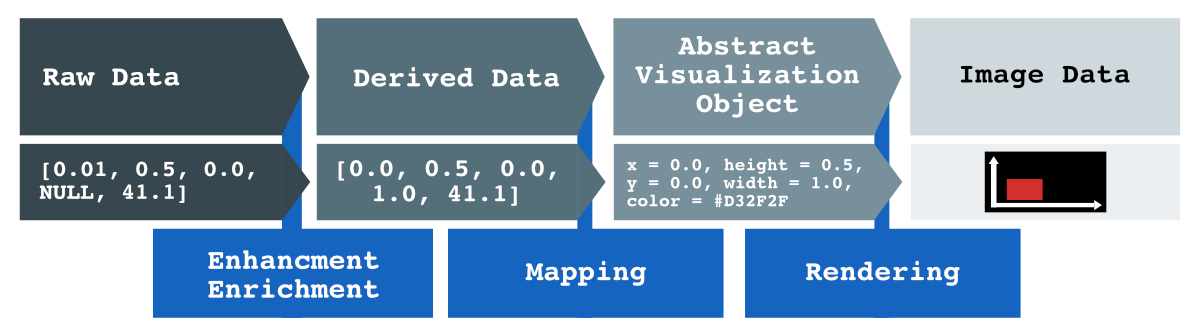
\includegraphics[width=15cm]{resources/img/VisualizationPipeline}
    \caption{Transformations and Resulting Data of the Data Visualization Pipeline}
    \label{fig:pipeline}
\end{figure}

The starting point of the pipeline is the raw data acquisitioned from a process
we are collecting data from. At this point the data has not yet been altered in
any way. The first transformation we execute on this data is an operation to
enhance or enrich the data. This can include interpolation for missing points in
the dataset or smoothing filters for noice in our dataset we want to get rid of.
In general, this step includes every calculation based on our raw dataset, which
is useful, but does not yet produce any visual information.  The resulting
dataset from this operation is called the derived data. 

The next transformation in the Pipeline is the mapping of the derived data onto
\glspl{avo}. These are not yet the image itself, but objects that describe the
later visual representation of an entry in the dataset using certain attributes.
An example for such an attribute could be a color, which is calculated from one
of the dimensions in derived data. An example for this transformation step would
be the mapping of a float value representing a measured temperature to a
corresponding color representing a specific temperature range.

The last step in the pipeline is the Rendering, which produces an actual pixel
image from the \gls{avo}. This step often involves operations from computer
graphics like transformations between object, scene and device coordinates. With
these transformations it is possible to produce a two dimensional pixel image of
an three dimensional scene. The rendering step of course depends highly on the
technologies used and the \glspl{avo} we want to display. Compared to other
usages of computer graphcis, the goal of rendering for data visualization is not
the production of a photo realistic image, but the creation of an abstract
approximation, that allows us to understand the scientific data it represents.
Unnecessary details would in this case only harm the performance of the pipeline
and distract the viewer. 

\cite{VisIdioms, UnderstDataThroughVis}

Based on this model, there are three different types of visualization software
systems. These different types of systems will bring different requirements to
each step of the pipeline.

The first type is used in situations, where the source for the data is run once
in the beginning, the data is collected and the visualization is done later.
This type of software is mainly used for visualizing results of experiments
running once without constant repetition. An example of such a system is the
acquistion of data coming from a particle detector. The recorded collision is
not something that will constantly be repeated over a long period of time, so
the main priority of performance is, that the storage system can keep up with
the high band-width data coming from the experiment. The visualization of such
data is often done on heavily filtered versions, that only take data into
account, which is interesting.

The second type of visualisation software systems are runtime monitoring
software. Compared to our first scenario, this software type requires all steps
of the pipeline to be completed more than once. As soon as new data gets
available from the source, it is passed through each step of the pipeline, to be
visualized at the end. One way to take load from a very work intensive step in
the pipeline, is to accumulate a certain amount of data before passing it onto
this step.

The third type of visualisation software allows the conductor of the source, to
interactively influence its execution. This means, that a runtime monitoring
system is extended using inputs, which allow the interaction between user and
data source. If the user sees problems rising while monitoring the process, he
can use the inputs provided by the software system to alter the the input
parameters. The success of the changes can be actively monitored while it is
running.

\cite{VisIdioms}

All of these three types of applications can be found to a certain extend at
\gls{cern}. In the next section we will have a look, how such sofware sytems are
used in a real scientific environment.


%% ==============================================
%%              Charting at CERN
%% ==============================================

\subsection{Charting at CERN}
\label{sec:fundamentals:cerncharting}

\begin{figure}[h]
    \centering
    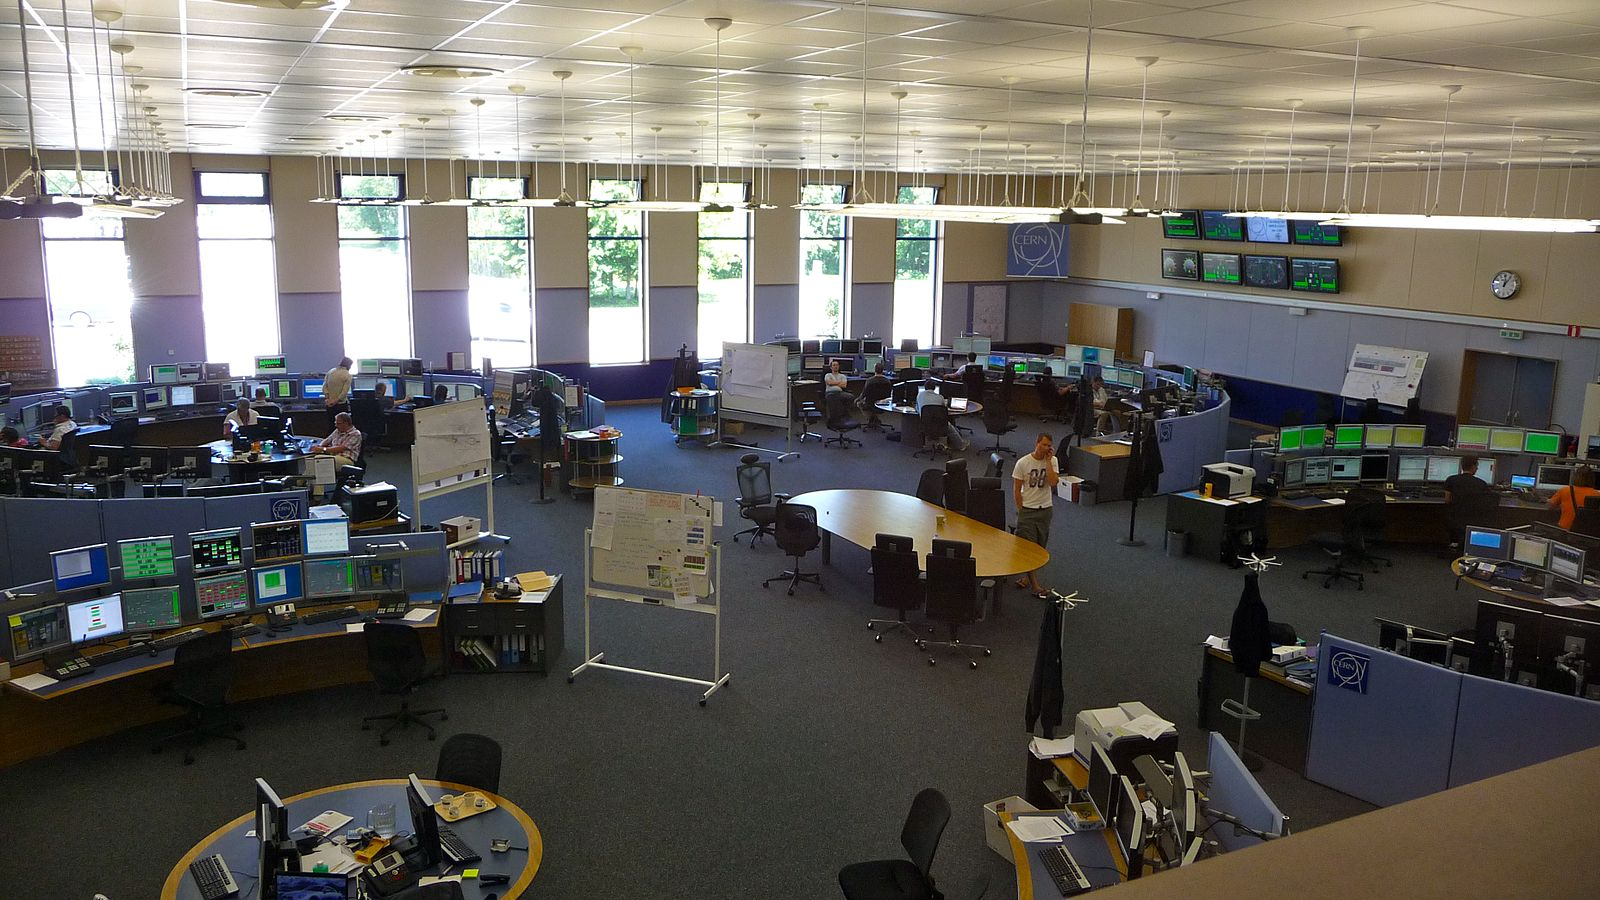
\includegraphics[width=14cm]{resources/img/CernControlCenter}
    \caption{CERN Control Center}
    \label{fig:ccc}
\end{figure}

Visualization Software Systems of the first type can be found at CERN for
example in the experiments using one of \gls{cern}'s particle detectors. During
Run 2, which lasted for four years and ended in Octobter 2018, all four
experiments produced around 25 Gigabytes of data per second. Even for the most
modern storage solutions, storing such a band-width of data is a unrealistic
challange. This would require massive amounts of high performance storage
devices, which would be a prohibitively expensive solution. To reduce the amount
of storage space needed, the Atlas Experiment filters out around 99 percent of
data in a two-step filtering process and only leaves the most promising events.
The actually stored data can then be analysed and visualized offline. One
example for such a display is a three dimensional view of recorded collisions in
the ATLAS Control room, which can be followed live online, if the detector is
running.

\cite{LhcDataStorage, LhcRun2, AtlasLiveCollisions, AtlasTrigger}

Implementations of the second and third type of data visualization software
systems can be found as well at \gls{cern}, especially for monitoring
continously running processes. One of these places is the \gls{ccc}, which's
main purpose is the monitoring of the accelerator complex. Operators, experts
for components of the complex, work here around the clock, to make sure that all
of them are runnning as expected. The \gls{ccc} is set up from four circular
areas called \emph{islands}, which are dedicated to monitor different parts of
the accelerator complex. These parts are the \gls{ti}, \gls{ps}, \gls{sps} and
\gls{lhc}. Collecting all of them under one roof allows them to directly keep
contact with each other making communication between them more efficient.

\cite{DayInCCC}

Consoles are computers in the \gls{ccc} that allow interaction with the
accelerator complexes control system through \glspl{gui}. Operator's Consoles
are used for setting parameters of components in the control system. \gls{gui}
applications running on these machines can be categroized as the inputs of data
visualization software systems of the third type.  Next to Operator Consoles
there are big wall mounted displays called Fixed Displays or Vistars, which are
running runtime monitoring applications in the form of dashboards, which allow
operators to monitor the status of a specific component of the accellerator
complex and see the resulting behavior of their interaction. Since they do not
allow any direct interaction, Fixed Displays can be categorized as visualization
applications of type two.

\cite{ControlSystemBible}

\begin{figure}[h]
    \centering
    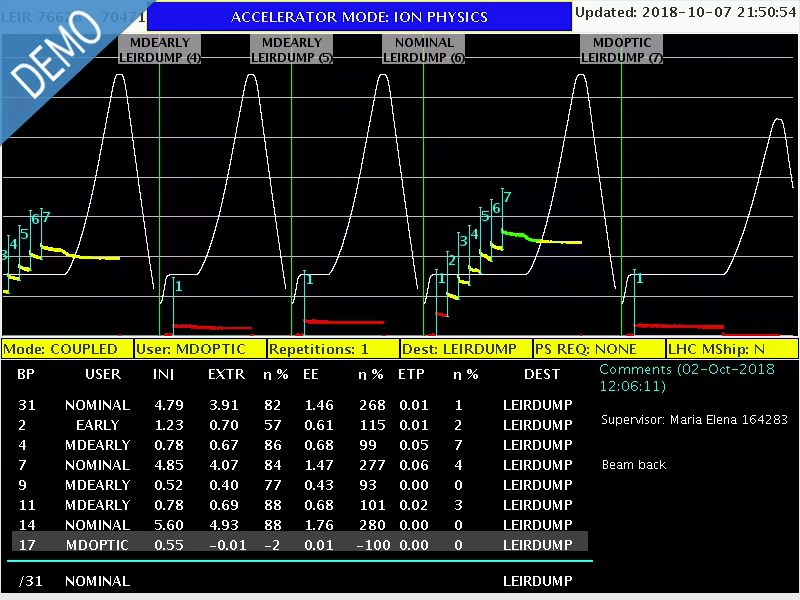
\includegraphics[width=12cm]{resources/img/LEIRVistar}
    \caption{LEIR Vistar in the \gls{ccc}}
    \label{fig:leir}
\end{figure}

One Vistar used as reference for the feature development of a graph library for
PyQt was the LEIR Vistar. LEIR is \gls{cern}'s Low Energy Ion Ring, which is
responsible for transforming a longer bunch of lead ions into shorter ones,
preparing them for the injection into the \gls{lhc}. Its Vistar contains a graph
at the top displaying the injection of particles, the energy level and the
different cyles.

\cite{Leir}




%% ==============================================
%%                  JDataViewer
%% ==============================================

\subsection{JDataViewer}
\label{sec:fundamentals:cerncharting:jdataviewer}

Fixed displays and \gls{gui} applications running on an Operator Console are
built using components provided by \gls{aps}. Previous to PyQt, \gls{aps}
focused mainly on Java and Swing to develope graphical user interfaces.
JDataViewer is a powerful library that allowed users to easily create charts and
interact with them. The library was developed in house at \gls{cern}, since
products on the market at that time were satisfying the charting needs of the
users. One feature, which seperates JDataViewer from the rest of libraries on
the market, is its capabilities, to use charts for editing the underlying data
set it is representing. Additionally to its large offerings in Features,
JDataViewer provides class leading performance when used in runtime monitoring
applications. Goal for its PyQt predeccessor is to offer similar features and
performance.

\cite{JDataViewer}


%% ==============================================
%%              Charting at CERN
%% ==============================================

\section{Benchmarking}
\label{sec:fundamentals:benchmarking}

The main advantage that invention of computers introduced into our lives was the
massive increase in speed and the possibility to automate tasks, which would
have taken us a time to complete in the past. Since then, computing speeds have
increased drastically over time. According to Gordon E. Moore, cofunder of
Intel, one of the world's largest semiconductor chip manufacturer, the
transistor count in a dense integrated cicuit doubles every second year. While
this does not mean, that computing power doubles exactly in the same way, it
shows us roughly, with which speeds computing power is increasing. Even with
these developments, we still can easily find computing tasks, that can take
modern computers a lot of time to complete, especially with a large amount of to
be processed data.

One way of handling highly complex computing tasks is to acquire more powerful
hardware, which can proccess more quickly through the given data. This appoach
harbors a simple problem, because the hardware we are able to acquire is often
bound to a specific budget. Since more computing power will inevitably mean a
higher count of transistorsn cores and clockspeeds, the price of hardware will
raise with its computing power. A less costly approach is the optimization of
the software which is used to perform a task. By utilizing the power of our
hardware more efficienlty, we can achieve the same results with less powerful
hardware. These two options lead to the question, which hardware and software
combinations are performant enough to carry out the work we want. To answer this
question, we need a procedure, which allows us to analyse performance
objectively, to take a sound decision.

\cite{mooresLaw}

Benchmarking is a procedure which allows us to objectively compare the
performance of a system or process, to find out, which work loads they are
capable of handling. The usage of Benchmarking is not restricted to computing.
In the field of Performance Management, benchmarking is a popular approach to
evaluate the effectiveness of processes in a business. In journals testing new
computing hardware, you can often find results, which a tested hardware achieved
in common benchmarking applications to give the potential customer a way to
compare different offerings on the market.

\cite{BenchmPerfManagement}

This chapter will give a overview about different approaches on performance
evaluation in the world of computing.




%% ==============================================
%%        Synthetic Hardware Benchmarks
%% ==============================================

\subsection{Synthetic Hardware Benchmarks}

Hardware benchmarks can range from simple and synthetic sequences of operations
to much more complex application like benchmarks that try to test a components
performance in a much more real world test scenario.

Before synthetic benchmarking applications were a thing, manufacturers used
\gls{mips} as a measurment to desribe performance of their chips. This would
describe, how many machine instructions a chip could execute per second.
Additionally \gls{flops} were used to supplement the computing performance
description in \gls{mips}, since high numbers in \gls{mips} were often achieved
using less expensice integer operations. Until today, \gls{flops} can be found
as a performance description for computing hardware, especially for GPUs. The
GeForce RTX 2080, a to the time of writing very recent GPU from the GPU
manufacturer NVIDIA, can theoretically reach up to 10.6 \gls{tflops} or $10.6 *
10^{12}$ \gls{flops}.

\cite{heiseGtx2080}

The first ever program that was explicitly desgined to test the perfromance of
computer hardware was called Whetstone. The first version was published by H.J.
Curnow and B.A. Wichmann in 1976 and was written in Algol 60. The goal of
Whetstone was to test a hardware's performance without relying on any hardware
specific instructions by replacing them a collection of different higher level
operations containing integer arithmetic, floating pointer arithmetic, if
statements, calls and more, which we still use frequently in modern programming
languages. When executing the benchmark, all of these instructions were
repeatingly executed. By using different weights for different operations, the
results of the benchmark in the end could be described in a measurment called
\emph{Whetstone operations per second}.  Another early benchmark that resulted
from a library of linear algebra
subroutines was LINPACK, which measured a computers speed in solving operations
on matrices. The result of the benchmarks were published in \gls{flops}.

\cite{OverviewBenchmarks}

A more modern suite of benchmarking applications is provided by SPEC. Spec is a
non profit-organization which offers a standardized suite of benchmarks, that
can be used to evaluate hardware performance. A new focus that SPEC brough up
into the world of benchmarking, was the consideration of energy efficiency next
to performance as an interesting measurment.

\cite{Spec}

Although it plays a very large role in the performance of an application on a
specific system, hardware is not the only factor that we have to take into
consideration when talking about performance in computing. The second important
part is the Software. No matter how fast the provided hardware is, if the
running software is written without fully utilizing the hardware's capabilities,
the resulting experience will be bad.  Because of this another apporach to
benchmarking is Software Benchmarking.




%% ==============================================
%%           Software Benchmarks
%% ==============================================

\subsection{Software Benchmarks}

Next to benchmarking hardware, we can also measure the performance of software.
Beanchmarking software is executing the same task in different implementations
on the same hardware and compare the recorded results. One example of software
benchmarking is the comparison of different programming languages. The free
software project \emph{The Computer Language Benchmark Game} uses a set of
different algorithms to test the performance of different languages in
implementing this algorithm. There are no restrictions on how to implement the
solution as long as they withstand a set of unit tests, that make sure the
implementation is actually correct. A description of the different benchmarks,
the different implementations and the results archieved in each implementation
can be found on the projects official webpage.  Even though the results can hint
the performance capabilities of different languages, the project states, that it
is important to see them in context. The performance of these mostly synthetic,
very isolated operations are not capable of displaying the entire performance
capability of the langugage.
\cite{CompLangBenchmGame}




%% ==============================================
%%           Application Benchmarks
%% ==============================================

\subsection{Application Benchmarks}

For most modern hardware, measurments like \gls{flops} are not very helpful,
when choosing hardware or the speed of a certain programming language when
working with binary trees, when choosing a software to perform a certain task.
The tasks of which's performance we actually do care about, are very high-level
and can be divided into countless subroutines. Application Benchmarks allow us,
to investigate the performance in such high-level use cases, which give us a
much more realistic image of the performance of hardware in our later use cases.
Depending on the use case, there are many offerings in Application Benchmarking
Software on the market.

Especially in jourinalism about computer hardware you can find a very wide
spread usage of application benchmarks to describe the performance of new
realeased harware products and how they will perform compared to older models.
Very common are benchmarks, that will use mostly CPU or the GPU to perform tasks
that are very close to the use cases of the customers of the hardware products.




%% ==============================================
%%       Collection of Benchmarking Criteria
%% ==============================================

\subsection{Collection of Benchmarking Criteria}

No matter, which type of benchmark we have been looking at, they can all be
described through common criterias.

1) Bechmarks should be written in high-level programming languages. This allows
us to port them easily onto other hardware. It is often required to execute
benchmarks on different architectures.

2) To give us a realistic view on a machines performance, the Benchmark should
also representative to the task we want to perform later on the hardware.
Running rendering benchmarks on graphics hardware does maybe give us an
comparable number when it comes to rendering capabilities, but does for example
no help us, if we are looking for graphics hardware to execute a certain machine
learning task on it.The best benchmark would always be the users actual
application.

3) Another fundamental requirement of a benchmark is, that the benchmark should
be easily measureable. Only if we can measure the benchmark easily and reliably,
we can produce comparable numbers in the end. 

4) The last requirement for benchmarks is, that they are widely distributed. If
benchmarking results are only available for one certain piece of hardware, but
not for its competitors, we do not have any comparability between them.




%% ==============================================
%%       The Qt Application Framework
%% ==============================================

\section{The Qt Application Framework}
\label{sec:fundamentals:qt}

To effectively develop benchmarking tools for python graph libraries, we have to
understand the principles of the underlying \gls{gui} framework first, which in
our case is the Qt application framework. This chapter will present an
introduction into the core principles of it.




%% ==============================================
%%     Widgets, Layouts and Widget Hierarchy
%% ==============================================

\subsection{Widgets, Layouts and Widget Hierarchy}
\label{sec:fundamentals:qt:basics}

For the implementation of the Benchmarking Framework, we have to focus on a
\gls{gui} Framework, in which our widgets will be embedded and tested. Since
\gls{aps} has decided for Qt as the base for \gls{gui} applications, we will
take the same decision for our implementation. This chapter will give a general
introduction in the creation of \glspl{gui} with the help of Qt.

Qt is a C++ Framework for developing cross-platform applications. It is
currently maintained by the Qt Company and offers licences for commercial and
open source usage. Qt is not just a collection of GUI components, but a complex
and powerful application framework. It is devided into three main packages:

\begin{description}
    
    \item[QtCore] offers non \gls{gui} related Core functionalities for
        applications.  

    \item[QtGui] offers \gls{gui} related data wrapper
        classes and utlity functions.
    
    \item[QtWidgets] offers a collection of high level \gls{gui} widget and
        layout classes.  

\end{description}

\inlinecode{Python}{QtWidgets.QApplication} is the central application class in
Qt. Only one instance of it can exist at a time which represents the current
state of our Application, but does not yet represent any visual components like
windows. If we want to present a window to the user, one option is to use
\inlinecode{Python}{QtWidgets.QMainWindow}. One way to create a window
containing our GUI components in it, is to subclass QMainWindow. In this
subclass we will have access to all functionality of QMainWindow and its
subclasses. One of these functions is
\inlinecode{Python}{QtWidgets.QWidget.show()}, which will draw the window on the
display presenting it to the user. The last step of every Qt \gls{gui}
Application is to call \inlinecode{Python}{QtWidgets.QApplication.exec()}, which
will start the Main Event Loop of the Application. More information about this
Event Loop and its role will be discussed in
\ref{sec:fundamentals:qt:eventloop}.

The code example \ref{listing:fundamentals:qt:basicapp} shows these mentioned
steps in a running Qt Application written in Python Code. The window it is
producing is not yet containing any widgets, but has a custom window title set
to it. A simple application like this does only depend on classes from the
\inlinecode{Python}{QtWidgets} package.

\lstinputlisting[
    caption=Hello World Qt GUI Application written in Python,
    language=python, 
    label=listing:fundamentals:qt:basicapp
]{resources/code/pyqtapp.py}

It is worth mentioning two additional details in regards to example
\ref{listing:fundamentals:qt:basicapp}. The first is, that we are passing of
\inlinecode{Python}{sys.argv} to the QApplication constructor. This allows us to
define parameters for the QApplication when invoking the python application from
command line. The second one is, that we pass the return status from
\inlinecode{Python}{app.exec()} when exiting Python. This allows us for example
to mark our Python Application as failed, if the QApplication fails and exits
with an exit code unequal to zero.

To add content to out window, Qt offers the concept of widgets. The base class
for every widget is \inlinecode{Python}{QtWidgets.QWidget}. Next to QWidget, the
package QtWidgets offers many more ready to use widgets for many different
purposes. All common UI building blocks, like labels, checkboxes, comboboxes and
more can be found and added to a window. QWidget itself can also be used as a
wrapper around multiple other widgets. Each widget can be given a parent on
creation. Using this functionality, the user can define a tree like parent child
hierarchy for all widgets starting from the main window. A big advantage that
this hierarchy offers, is that with the deletion of a widget, all its child
widgets will be deleted as well.

Next to widget classes, Qt offers layout classes to order multiple children
inside a parent widget. Some very basic layouting options include:

\begin{description}

    \item \inlinecode{Python}{QtWidgets.QVBoxLayout} aligns widgets vertically
        below each other.
    
    \item \inlinecode{Python}{QtWidgets.QHBoxLayout} aligns widgets horizontally
        next to each other other.
    
    \item \inlinecode{Python}{QtWidgets.QGridLayout} aligns widgets in a grid.

\end{description}

Next to those basic ones, Qt also offers more complex ones with additional
functionality. Other options for layouting a window is grouping widgets into
containers using Container Widgets. As an example, the class
\inlinecode{Python}{QtWidgets.QTabWidget} allows grouping widgets into different
views, which can be switched between by clicking on differnt tabs. By utilizing
these different widgets and layout options, you can build more complex window
layouts as seen as seen visible in depiction \ref{fig:qt:examplewindow}. On the
right side of the depiction you can see the widget and layout types contained in
the result window visible on the left. The source code for this window is
appended in \ref{a:fig:qt:examplewindow:code}.  \cite{PythonGui1}

\begin{figure}[h]
    \centering
    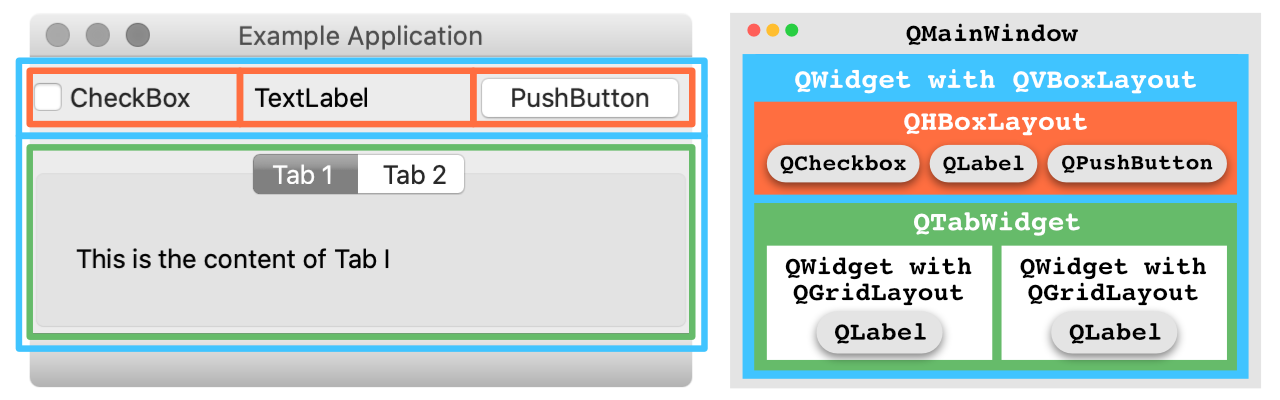
\includegraphics[width=15cm]{resources/img/QtExample}
    \caption{Layouts and Widgets in a Qt Application Window}
    \label{fig:qt:examplewindow}
\end{figure}

At this point, we have learned, how we can define the appereance of a \gls{gui}
application, but interacting with these components does not yet invoke any
logic. In the following section we will have a look, how we can attach logic to
the user interface components.


%% ==============================================
%%             Signals and Slots
%% ==============================================

\subsection{Signals and Slots}
\label{sec:fundamentals:qt:signalsslots}

At this point, all our examples for \gls{gui} applications have not yet been
very useful, since the interaction with elements does not yet invoke any
actions. For this we have to define a connection between user interface
components and a function, which implements the logic we want to invoke. Many
\gls{gui} Frameworks realise this connection through callbacks. A callback is a
pointer to a function, which is invoked, when intraction with a certain user
interface element is detected. One problem this approach harbors is, that with
callbacks it can't be ensured, that the passed arguments have the right type.

To solve this problem, Qt offers a concept called Signals and Slots for
communication between objects. All widgets from the package
\inlinecode{Python}{QtWidgets} do inherit from
\inlinecode{Python}{QtCore.QObject} and do offer different standard signals and
slots for informing about and reacting to state changes. The usage of Signals
and Slots is not restricted to the communication between \gls{gui} elements and
business logic, but can be used in any classes derived from
\inlinecode{Python}{QtCore.QObject}.

Signals are public functions, which emit messages informing about changes in the
state of the object who emitted them. Slots are simply normal instance methods
with the addition, that they can be connected to Signals to receive and react to
the messages sent from this Signal. Since they are normal instance methods,
Slots can also be called normally from code. The connection between both is set
up, by connecting a signal of an object to a slot of an object. A signal can be
connected to multiple slots and a slot can be connected to multiples signals.
Depiction \ref{fig:qt:signalsslots} shows a schema of an example scenario where
different objects are communicating using singals and slots.

\begin{figure}[h]
    \centering
    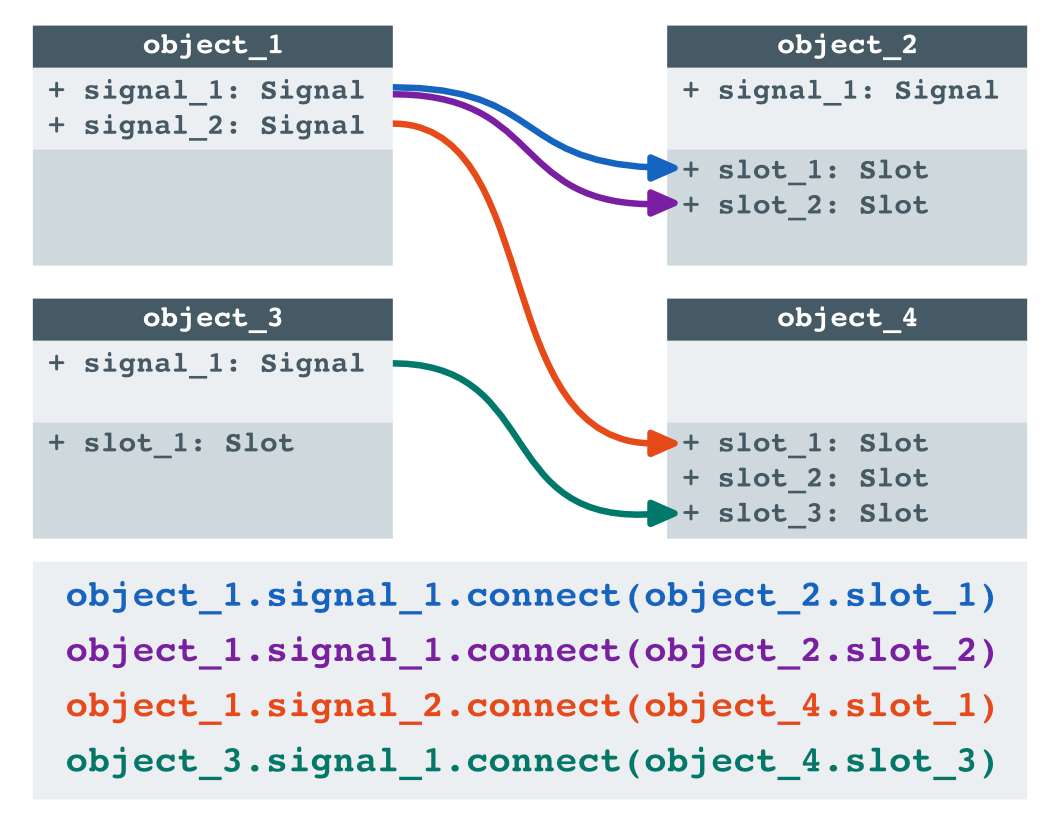
\includegraphics[width=12cm]{resources/img/QtSignalsSlots}
    \caption{Communication between objects through Signal and Slot Connections}
    \label{fig:qt:signalsslots}
\end{figure}

One big advantage of Signals and Slots is, that objects are fully independent
from each other, since neither the slots knows, which signals it is connected
to, nor the signals knows which slots it is connected with. Compared to
callbacks, the Signal and Slots have more Overhead, which makes their execution
slower. Compared to any f.e. List Operation requiring \inlinecode{C++}{new} or
\inlinecode{C++}{delete}, this overhead is still much smaller. In real life
applications, the perfromance losses coming through the usage of Signals and
Slots are insignificant.  \cite{QtSignalsAndSlots, PythonGui1}

Listing \ref{listing:fundamentals:qt:signalsslots} shows a simple scenario,
where the signal of a \inlinecode{Python}{QtWidgets.QLineEdit}, is connected to
a slot of a \inlinecode{Python}{QtWidgets.QLabel}. Both Singal and Slot are
already implemented in these classes and can be simply connected. If you change
the text in the line edit widget, the signal \inlinecode{Python}{textChanged}
will emit this new text, which the Slot \inlinecode{Python}{setText} receives
and displays.

\lstinputlisting[
    caption=Connecting items through singals and slots,
    language=python,
    label=listing:fundamentals:qt:signalsslots
]{resources/code/signals_and_slots.py}

In some cases, for example when we create own widgets, we have to define own
signals and slots. This is possible as well. For this we will extend our example
with another Label from our own type \inlinecode{Python}{WatchLabel} derived
from \inlinecode{Python}{QtWidgets.QLabel}, which offers a slot
\inlinecode{Python}{set_time}, that takes a float value, interprets it as a
timestamp and displays it. To update this label, we will introduce another
object \inlinecode{Python}{WatchTick} derived from
\inlinecode{Python}{QtCore.QObject}, which sends a signal 60 times per second
containing the current timestamp.
\ref{listing:fundamentals:qt:signalsslots:custom} shows the definition of these
two components. Since we have typing information in the signal and the slot
definition, Qt makes sure, that both will work together. If both types do not
match, a \inlinecode{Python}{TypeError} will be raised.

\lstinputlisting[
    caption=Defining a custom signal and slot,
    language=python,
    label=listing:fundamentals:qt:signalsslots:custom,
    firstline=2,
    lastline=33
]{resources/code/signals_and_slots_custom.py}

As in listing \ref{listing:fundamentals:qt:signalsslots}, we can simply connect
the new slot with the signal. After starting the timer, the signal will be
emitted aroung 60 times per second, which will update the label, which then
shows the current time.

\lstinputlisting[
    caption=Using custom Signals and Slots,
    language=python,
    label=listing:fundamentals:qt:signalsslots:custom:connect,
    firstline=42,
    lastline=46
]{resources/code/signals_and_slots_custom.py}

Since Qt Applications are event driven, they can be created as a single threaded
application without any problems. In more complex applications, some operations
can take a bit of time to complete, which, when executing in the main \gls{gui}
Thread, would block all interaction with the user interface. To keep the
\gls{gui} responsive, work intensive operations can be moved to a seperate
Thread for parallel execution using for example Qt's
\inlinecode{Python}{QtCore.QThread}. Signals and Slots offer a very convenient
way to communicate between these multiple Threads. An example for that would be,
that the \gls{gui} Thread spawns a new Worker Thread, in which a computing
intensive process is running. If finished, this worker thread can inform the
\gls{gui} Thread about its completion by emitting a signal, which can then
display the results from the worker thread.

When working with multiples Threads in a Qt Application, it is important to know
about the different connection types which Qt offers. These connection types
control, when and in which Thread the connected slot is executed. A
\inlinecode{C++}{QtCore.Qt::DirectConnection} for example leads to the Slot
being executed directly in the Thread of the emitting object. Between the Signal
being emitted and the Slot being called, the control is not given back to the
event loop. A \inlinecode{C++}{QtCore.Qt::QueuedConnection} on the other hand
executes the Slot in the Thread where the receiving object lives. With this
type, the control is returned to the event loop. The default connection type
\inlinecode{C++}{QtCore.Qt::AutoConnection} will decide between queued and
direct connection depending on in which Thread the emitting and receiving object
are living.

\cite{QtConnectionTypes}




%% ==============================================
%%             The Event System
%% ==============================================

\subsection{The Event System}
\label{sec:fundamentals:qt:eventloop}

Qt Applications can very often be written without using parallel programming at
all, which vastly decreases the complexity of the application and increases
maintainability. Qt is an event-driven toolkit, which means, that applications
are designed to wait for events and react to them appropriatly. In general
Events can be described as anything which has happened, which the application
has to know about.  These Events can be Mouse Clicks, Timer Timeouts or internal
events which are supposed to tell a part of the \gls{gui} to redraw. Events can
also come from different places: Mouse Click or Key Events are most likely
coming from the Window Manager while other events can come either from the
application code or the Qt Framework.
Qt does not necessarely handle events immediately as they arrive, but queues
them for later handling. The Qt Event Loop is responsible for iterating over
these queued Events posted to the Event Queue to process them accordingly.

If we have a look at the examples in section \ref{sec:fundamentals:qt:basics},
we will see a the line \inlinecode{Python}{app.exec()} in them. This call will
start Qt's Event Loop and will be blocking until the application terminates.
Code placed below this line will only be evaluated when the application has
already quit. This means, that operations for showing a window or adding widgets
to it will have to be placed above it. After the main event loop is started, it
will retrieve events from the queue and process them one by one. Prior defined
operations for showing window or adding content to it are for example such
Events. In Qt all these events are packaged into a class derived from
\inlinecode{Python}{QtCore.QEvent}. A \inlinecode{Python}{QtGui.QMouseEvent} for
example is derived from it and extends it with functions specific to this type
of Event like \inlinecode{Python}{QtGui.QMouseEvent::buttons()}, which returns
information about buttons that were pressed during this Event.

To make sure that Events are properly processed, they have to be published to
the Event Loop and the Event Queue. While such events can appear from outside
the application code, they can also be created and published within it. To
create an Event, an instance of the fitting Event Type has to be created. As
mentioned, for standard Event types, Qt offers already implemented classes.
Events can be published either through
\inlinecode{Python}{QtCore.QtCoreApplication.sendEvent()} or
\inlinecode{Python}{QtCore.QtCoreApplication.postEvent()}. 

The first will lead to immediate delivering and handling of the Event without
any involvment of the Event Loop, while the later one will add the Event to the
Event Queue, from where it will be deliverd by Qt when it is its turn. Listing
\ref{listing:fundamentals:qt:eventcreation} shows as an example the creation of
a Mouse Press Event for a Click with the Left Mouse Button and its propagation
to a widget contained in the window. The widget which receives the Event is a
widget derived from \inlinecode{Python}{QtWidgets.QLabel}, which does not yet
change its state in any way when receiving Mouse Press Events.

\lstinputlisting[
    caption=Positing a MousePressEvent to a Widget,
    language=python,
    label=listing:fundamentals:qt:eventcreation
]{resources/code/event_sending.py}

When it is time to process an Event, Qt delivers them to widgets, so they can
react to them if they want. The type of the Event does also influence in which
way it is delivered. If a event is not accepted by a child widget, it is
propagated to its parent widget, where this principle repeats. If an event is
accepted by a widget and how the widget reacts to it, is defined in a Widgets
Event Handler.

Widgets have two options when defining their behavior on the delivery of Events.
The first option to handle arriving Events is
\inlinecode{Python}{QtCore.QObject.event()}, which is the general event handler
for all kinds of events. Here it is possible to intersect events of a specific
type. For all other events your widget does not care about, the base classes
implementation of \inlinecode{Python}{event()} can be called. Listing
\ref{listing:fundamentals:qt:eventhandler:one} shows the implementation of a
label class derived from \inlinecode{Python}{QtWidgets.QLabel}, which accpets
Mouse Click Events. If the widget detects a Mouse Click Event, it accpets it and
increases it Font Size by one point.

\lstinputlisting[
    caption=Change Font Size through Mouse Press using General Event Handler,
    language=python, 
    label=listing:fundamentals:qt:eventhandler:one
]{resources/code/event_handler_1.py}

If the widget is only supposed to handle specific types of Events, more specific
Event Handlers can be overwritten. Listing
\ref{listing:fundamentals:qt:eventhandler:two} shows the same Use Case as before
but achieved through overwriting the specific event handler dedicated to Mouse
Button Clicks.

\lstinputlisting[
    caption=Change Font Size through Mouse Click using Mouse Press Event Handler,
    language=python, 
    label=listing:fundamentals:qt:eventhandler:two
]{resources/code/event_handler_2.py}

Which events are delivered to which widgets, is decided by Qt, where different
Factors can play a key role. For the Mouse Click Events the position of the
pointer at the time of the Event does play a key role. Qt also offers the
possibility to install global Event Filters which allow us to filter out events
we do not like our Widgets to receive. These Filters are simply classes derived
from \inlinecode{Python}{QtCore.QObject}, which implement the
\inlinecode{Python}{QtCore.QObject.eventFilter()} protected method. This Event
Filter can then be intalled on any \inlinecode{Python}{QtCore.QObject} and is
working for it and its children. To install it globally for the whole
application, it cann be installed on the
\inlinecode{Python}{QWidgets.QApplication} instance as you can see as an example
in listing \ref{listing:fundamentals:qt:eventfilter}. As before, we have to
return \inlinecode{Python}{True} to prevent Qt from further propagating the
event to other widgets.

\lstinputlisting[
    caption=Installing an application wide event filter for single and double mouse button presses,
    language=python, 
    label=listing:fundamentals:qt:eventfilter
]{resources/code/event_filter.py}

Listing \ref{a:qtevents:code} contains a runnable application which demonstrate
these three concepts of event creation, even handling and event filtering in a
single simple application window similar to the here shown code snippets. It
contains two labels reacting to mouse clicks by changing their font size, a
button sending a mouse press events to both labels and a checkbox which installs
an EventFilter for Mouse Clicks on Labels and removes it again when unchecked.
\cite{EventSystem,AnotherLookAtEvents,EventFilters}




%% ==============================================
%%             Python bindings
%% ==============================================

\subsection{Python bindings}
\label{sec:fundamentals:qt:pyqt}

Even though we do now have a basic understanding about the fundamental
pronciples of the Qt Framework, we have not yet mentioned, how we can use a C++
application Framework in Python Code. This is possible through a principle known
as Python bindings and is not exclusive to the Qt Application Framework. Python
Bindings allow you to write Applications in Python using already existing C and
C++ libraries, which are already well received and popular. One very popular
Python Binding for the Qt Application Framework is PyQt, developed by Riverbank
Computing Limited. Riverbank provides different versions of PyQt for different
versions of Qt, for Qt5 we will pick PyQt5, which is the most recent version of
PyQt.  \cite{PyQtIntro}

Qt is a big Framework containg over one thousand classes, which have to be
accessible through Python to reflect the complete set of Features. It is
generally possible to write these bindings by hand, but a lot of work. To
automate the creation of Python Bindings, Riverbank has developed the tool SIP,
which can generate such Python bindings from interface header files with simliar
syntax to C++ header files. These files define what classes and methods should
be exported and how to call the module it should be exported into. Additionally
it is possible to define the translation between Python and C++ Objects.  SIP
then takes this header file and generates C++ Code, which can then be compiled
to an extension module for the Python Interpreter. These Extension Modules allow
us to import and call C and C++ libraries within our Python Code, which in the
Case of PyQt is the underlying Qt Framework.
\cite{SipIntro, SipTut, ExtendingPython}

Working with a C++ library comes with a few caveats which we will have to keep
in mind especially when working with the Qt Framework from Python. One
particular caveat, which can easily lead to Errors, is, that Objects do exist
not only as Python objects, but as C++ objects as well, which the Python object
is referencing. Qt on the other hand has its own Garbage collection mechanism,
which can delete objects if their parent object is deleted or if they do not
have any parent object. This deletion does not influence the existance of the
object on the Python side in any way, which makes it possible trying to access a
deleted C++ objects through their Python references, which will raise Runtime
Errors. When trying to delete a widget, it is also not enough to delete the
Python object with \inlinecode{Python}{del self.my_widget}, since the C++
underneath can exist further. Not being aware of this can easily create
applications with severe memory leakage, especially when creating and deleting
repeatadly new widgets, for example when opening new dialogs in an application.
To free the memory occupied by an widget's C++ object, we have to tell Qt, as
seen in listing \ref{listing:fundamentals:qt:objectdeletion}, to delte the
object and its children.

\begin{lstlisting}[
    caption=Example for properly deleting a QWidget,
    language=python, 
    label=listing:fundamentals:qt:objectdeletion
]
self.my_widget = QWidget(parent=other_widget)
# Posts an event to Qt's Event Loop to delete the object
self.my_widget.deleteLater()
# optionally we can delete the python referece now
del self.my_widget
\end{lstlisting}

Another caveat when working with PyQt is, when working with different Threads.
When working for example with \inlinecode{Python}{QtCore.QThread} on the C++
side, execution can be truely parallel on multi core systems. Working with
different threads in Python is possible as well, but if a
\inlinecode{Python}{QtCore.QThread} runs CPU bound Python Code like complex
calculations, it won't be executed parrallel on systems which would support true
parallel execution. The reason for this is Python's \gls{gil}. The \gls{gil} was
introduced to python for memory management reasons to keep track of object
references. Before a thread accesses any Python objects, it has to hold this
lock, which means, that code running inside the \gls{gil} can't take real
advantage of Multi Core Systems.

\cite{PythonGil, PythonGilDocs}

Since PyQt5 is not the only available Python binding for Qt, we will use the
Python package \inlinecode{Python}{qtpy} for all our code, which is a simple
pure Python abstraction layer, which will delegate all imports to whatever
Python binding for Qt is installed. This has the big advantage, that the code,
we developed with PyQt5, will run also in environments which have for example
the Qt binding PySide or PyQt4 installed. Listing
\ref{listing:fundamentals:qt:qtpy} shows those two options.

\begin{lstlisting}[
    caption=Qt imports using qtpy instead of a python library,
    language=python, 
    label=listing:fundamentals:qt:qtpy
]
# Direct usage of a Python binding, will fail if environment doesn't use PyQt5
from PyQt5 import QtCore, QtGui, QtWidgets
# Using qtpy for Qt related imports, will work with PyQt and PySide
from qtpy import QtCore, QtGui, QtWidgets
\end{lstlisting}

